\subsection{Forwards and Futures}

\subsubsection{Pricing}



\subsubsection{Hedging with Futures}

The fundamentals of hedging with futures are \hlt{hedge-and-forget} strategies, where no changes is made to adjust the hedge once it has been put in place.

\begin{definition}
\hlt{(Basic Principles of Futures Hedging)}\\
The objective is to take a position that neutralises the risk as far as possible.
\begin{enumerate}[label=\roman*.]
\setlength{\itemsep}{0pt}
\item \hlt{Short Hedge}: short position on futures. \\
Used when hedger already owns an asset and will sell the asset at some time in the future; or when asset is not owned right now but will be owned and ready for sale sometime in the future.
\item \hlt{Long Hedge}: long position on futures. \\
Used when hedger will purchase an asset in the future and wants to lock in the price now.
\end{enumerate}
\begin{table}[h]
\begin{tabular}{|c | c | c|}
\hline
 & \textbf{Short Hedge} & \textbf{Long Hedge} \\ \hline
May $15$ & \makecell[l]{Spot: $50$ \\ Futures: $49$} & \makecell[l]{Spot: $50$ \\ Futures: $49$} \\ \hline
August $15$ Scenario 1 & \makecell[l]{Spot: $45$ \\ Gain from hedge: $4$} &  \makecell[l]{Spot: $45$ \\ Loss from hedge: $4$} \\ \hline
August $15$ Scenario 2 & \makecell[l]{Spot: $55$ \\ Loss from hedge: $6$} & \makecell[l]{Spot: $55$ \\ Gain from hedge: $6$} \\ \hline
\end{tabular}
\end{table}
\end{definition}

In practice, hedging is not perfect due to factors as follows:
\begin{enumerate}[label=\arabic*.]
\setlength{\itemsep}{0pt}
\item Asset being hedged is not exactly the same as the asset underlying the futures contract.
\item Uncertainty as to exact date in which the asset will be bought or sold.
\item Hedge may require the futures contract to be closed out before its delivery month.
\end{enumerate}
These lead to \hlt{basis risk}.

\begin{definition}
The \hlt{basis} in a hedging situation is defined as
\begin{align}
\text{Basis} = \text{Spot Price} - \text{Futures Price} \nonumber
\end{align}
An increase/decrease in basis is a strengthening/weakening of the basis.
\end{definition}

\begin{definition}
Let $S_i$ be spot price at time $t_i$, $F_i$ be futures price at time $t_i$, $b_i$ be basis price at time $t_i$.	 Assume hedge is placed at time $t_1$, closed at time $t_2$. Price realised for asset is $S_2$, profit from futures position is $F_1 - F_2$.  Effective price obtained for asset hedging is therefore $S_2 + F_1 - F_2 = F_1 + b_2$.\\
If $b_2$ is known, perfect hedge will result. The \hlt{basis risk} is the hedging risk from uncertainty associated with $b_2$.
\end{definition}

\begin{definition}
\hlt{Cross Hedging} occurs when the asset underlying the futures contract is not the same as the asset whose price is being hedged.
\end{definition}

Cross hedging is often used when futures of the original asset being hedged are not actively traded on the market, and the hedger seeks an alternative asset to hedge the original asset.

\begin{definition}
\hlt{Hedge Ratio} is the ratio of size of position taken in futures contract to the size of exposure.
\end{definition}

Assuming no daily settlement of futures contracts, hedger seeks a hedge ratio that minimises variance of hedged position value. Let $\Delta S$ be change in spot price, $\Delta F$ change in futures price. Assuming linear relationship,
\begin{equation}
\Delta S = a + b \Delta F + \epsilon	 \nonumber
\end{equation}
where $a,b$ are constants, $\epsilon$ is an error term. Suppose hedge ratio is $h$. Change in value of position per unit of exposure to $S$ is:
\begin{equation}
\Delta S - h \Delta F = a + (b-h) \Delta F + \epsilon \nonumber
\end{equation}
Standard deviation is minimised by setting $h=b$. Let minimum variance hedge ratio be $h^*$. Then
\begin{equation}
h^* = \rho \frac{\sigma_S}{\sigma_F} \nonumber
\end{equation}
where $\sigma_S, \sigma_F$ is standard deviation of $\Delta S, \Delta F$ respectively, $\rho$ is coefficient of correlation.

\begin{figure}[H]
\centering
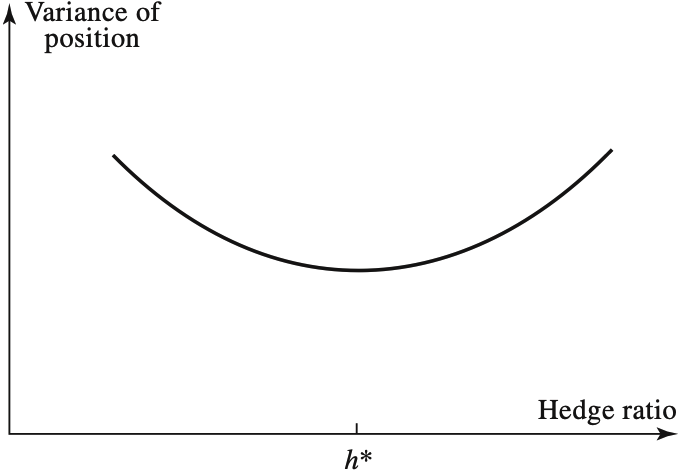
\includegraphics[scale=0.5]{derivatives/hedgeratio}
\caption{Dependence of variance of position on hedge ratio.}
\end{figure}

\hlt{Hedge effectiveness} is the proportion of variance eliminated by hedging. This is $R^2$ from regression of $\Delta S$ against $\Delta F$, and equals $\rho^2$. Parameters $\rho$, $\sigma_S$, $\sigma_F$ are estimated from historical data on $\Delta S$ and $\Delta F$.\\

The optimal number of futures to be used in hedging is
\begin{equation}
N^* = \frac{h^* Q_A}{Q_F} \nonumber
\end{equation}
where $Q_A$ is size of potion being hedged (units), $Q_F$ is size of one futures contract (units). The futures contract should be on $h^* Q_A$ units of the asset.\\

If daily settlement is used, there are a series of one-day hedges, and thus let $\hat{\sigma}_S, \hat{\sigma}_F$ be standard deviation of percentage one-day changes in spot and future price respectively, $\hat{\rho}$ be correlation between percentage one-day changes in spot and future prices. The optimal one day hedge is then
\begin{equation}
h^* = \hat{\rho}\frac{\hat{\sigma}_S S}{\hat{\sigma}_F F} \nonumber
\end{equation} 
and the optimal number of futures to be used is then
\begin{equation}
N^* = \hat{\rho}\frac{\hat{\sigma}_S S Q_A}{\hat{\sigma}_F F Q_F} \nonumber
\end{equation}

If an interest $r\%$ per annum is earned or paid over the remaining life of the hedge, then the optimal number of futures is $N^* / (1+0.01r)$; this is \hlt{tailing the hedge}.\\

Stock index futures may be used to hedge a well diversified equity portfolio. Let $V_A, V_F$ be the current value of portfolio and one futures contract respectively.\\
If portfolio mirrors the index, the optimal hedge ratio is then $1.0$, and number of futures contracts to be shorted is then $N^* = \frac{V_A}{V_F}$. If portfolio do not mirror the index, then capital asset pricing model (CAPM) should be used to determine beta ($\beta$), and the number of futures contracts to be shorted is then $N^* = \beta \frac{V_A}{V_F}$, assuming maturity of futures contract is close to the maturity of the hedge.\\

If instead, the hedger wishes to change the beta of portfolio where $\beta > \beta^*$, a short position $(\beta - \beta^*)\frac{V_A}{V_F}$ is required. If $\beta < \beta^*$, then a long position $(\beta^* - \beta)\frac{V_A}{V_F}$ is required.\\

Stock index hedging is typically used when the portfolio manager is uncertain about performance of market, but is confident that the stocks in the portfolio will outperform the market. The hedger may also be planning to hold a portfolio for a long period of time and requires short-term protection in an uncertain market situation.\\

If expiration date of hedge is later than delivery dates of all futures contracts that may be used, then the hedger may \hlt{stack and roll} by closing out one futures contract and taking the same position in a futures contract with a later delivery date.



